%
%  hubcheck.tex  2012-04-09  Derrick Kearney
%
%  Describe what hubcheck is and the pieces that make it up.
%

%\setenumerate[1]{label=\Roman*.}
%\setenumerate[2]{label=\Alph*.}
%\setenumerate[3]{label=\roman*.}
%\setenumerate[4]{label=\alph*.}
%\begin{outline}[enumerate]

%\1 Selenium WebDriver
%  \2 Abstracts web browser automation.
%  \2 Focused on reproducing how a user interacts with the web page.
%  \2 Support actions like clicking on element, typing in inputs, moving
%     the mouse pointer.
%  \2 Relies on web browser to execute javascript.
%  \2 Works with Firefox, Opera, IE, PhantomJs, Safari, Mobile browsers, others.
%  \2 Runs in remote server mode or local mode.
%  \2 Controls starting a new web browser for each test case.
%  \2 User can send commands to browser using Java or other languages
%     through a RESTful, JSON based, remote wire protocol web service.
%  \2 Results of commands are sent back to user, through the programming language,
%     for processing.
%\1 BrowserMob Proxy
%  \2 Built to capture performance data for web applications
%  \2 Can be used to record, redirect, and block http and https requests.
%  \2 Records HTTP Archive (HAR) which provides HTTP status codes,
%     along with request/response timings among other things.
%  \2 Provides information about requests that are not provided by
%     Selenium WebDriver. Selenium WebDriver wants to stay focused
%     on user interactions.
%\1 Paramiko
%  \2 Python module that implements the SSH version 2 protocol
%  \2 Allows for creating SSH and SFTP connections for secure connections
%     to remote machines.

\chapter{EXTERNAL LIBRARIES}
\label{chap:external_libraries}

HUBcheck builds upon several external libraries to provide web browser and
shell based automation. To support web automation, HUBcheck uses the Selenium
WebDriver API \cite{SeleniumWebDriver:Online} and the BrowserMob Proxy
\cite{BrowserMOBProxy:Online}. The WebDriver API is used to control the web
browser and is provided by the Selenium project along with bindings for several
programming languages. The BrowserMob Proxy is an open source web proxy,
maintained by Patrick Lightbody, which can be used to watch and manipulate
network traffic. To support shell automation, HUBcheck builds upon Paramiko
\cite{Paramiko:Online}, a Python implementation of the SSH version 2 protocol.
Below we'll learn more about the role each of these libraries plays.

\section{Selenium WebDriver}
\label{sec:external_libs_selenium}

% describes the webdriver api
% http://www.w3.org/TR/webdriver/

% describes the firefox driver
% http://code.google.com/p/selenium/wiki/FirefoxDriver

Selenium is an open source project with a suite of tools used to automate web
browsers across many platforms. Selenium implements the WebDriver API as a part
of the Selenium WebDriver library. The WebDriver API provides an
object-oriented programming interface to communicate with and control a web
browser, performing the same actions a person would when interacting with a web
page.  Through the WebDriver API, developers can launch a web browser, locate
elements in web pages, and perform actions on elements such as typing into them
or clicking on them using the mouse. The following subsections show examples of
how Selenium WebDriver can be used to control a Firefox web browser using the
Python programming language.

\subsection{Launching a Web Browser}
\label{ssec:external_libs_selenium_launch_browser}

The Selenium WebDriver Python bindings provide the \xfmodule{webdriver}
module that holds classes to represent the different types of browsers that
can be launched, including Firefox, Chrome, Safari, Opera, and PhantomJS.
Browsers can be launched locally on the same machine running the automation
program, or on a remote host that is running a Selenium Server. Each browser
has a special plugin which translates the WebDriver requests,
made from Selenium, to the browser's native automation API.

Launching a web browser using Selenium is as simple as instantiating a new
\xfobject{webdriver} object for the browser the user wants to launch. With no
initialization arguments, the user will be provided with a new browser they can
control by calling member functions of the returned object as demonstrated in
\Cref{lst:selenium_launch_browser}.


\begin{xcode}{%
  language=Python,%
  label=lst:selenium_launch_browser,%
  caption={Launching a locally hosted Firefox web browser using Selenium WebDriver's Python API},%
}
from selenium import webdriver

browser = webdriver.Firefox()
browser.get('https://hubzero.org')
\end{xcode}


%Properties of the web browser and desired system to host the browser can be
%passed to the driver. This is useful when automating in an environment where
%multiple web browsers or host systems are available. Browser capabilities
%include items like the host platform, file paths to browsers, and
%expressing operating system requirements. \Cref{fig:capabilities_setup}
%shows how to setup a capabilities dictionary to start the Firefox browser on a
%Debian/Linux system using the Python programming language.
%
%\begin{xcode}{%
%  language=Python,%
%  label=lst:capabilities_setup,%
%  caption={The capabilities dictionary is used to tell the driver program what system properties are desired for the browser that is about to be launched.}%
%}
%capabilities = {}
%capabilities['platform'] = 'ANY'
%capabilities['browserName'] = 'firefox'
%capabilities['version'] = ''
%capabilities['javascriptEnabled'] = True
%capabilities['firefox\_binary'] = '/usr/bin/firefox'
%\end{xcode}


For some browsers, more fine grained web browser controls are exposed to the
developer through access to the browser's profile.  Not all browsers support the
profile concept. Firefox allows users to load a pre-configured profile or
create one on the fly.

\begin{xcode}{%
  language=Python,%
  label=lst:firefox_profile_example,%
  caption={Adjusting the preferences in the Firefox browser.}%
}
from selenium import webdriver

profile = webdriver.FirefoxProfile()
profile.set_preference('browser.startup.page',0)
profile.set_preference('app.update.enabled','False')
profile.add_extension('firebug-1.11.4.xpi')
profile.set_preference('extensions.firebug.currentVersion','1.11.4')

browser = webdriver.Firefox(firefox_profile=profile)
browser.get('https://hubzero.org')
\end{xcode}

\Cref{lst:firefox_profile_example} demonstrates setting up a Firefox
browser profile that disables the startup page, disables automatic updates to
the browser, and installs the Firebug browser extension.  The FirefoxProfile
class allows developers to set preferences and add extensions to the Firefox
browser. Alternatively, users can take advantage of the class's
\xfparameter{profile\_directory} argument to load a pre-configured browser
profile.

The \xfclass{webdriver.Firefox} class is used to launch the web browser. If a
custom profile was created it can be provided to the class and a web browser
based on those settings will be started. The object returned, shown in line 9
of \Cref{lst:firefox_profile_example}, is stored in the variable
\xfparameter{browser}, and is used in automation scripts as the object
reference for the web browser. All commands to the web browser, such as
navigation and locating web elements in the HTML DOM (Document Object Model),
are performed on the \xfparameter{browser} variable using the \xfmethod{get()}
and \xfmethod{find\_element()} family of methods.

\subsection{Locating Elements on the Web Page}
\label{ssec:external_libs_selenium_locating_elements}

%The first step to doing anything interesting with a web page is to be able to
%locate HTML elements on the web page. The \textit{browser} object provides 6
%variations of the \textit{find\_elements()} method to help the user located
%HTML elements. Each variation allows the automation developer to use a
%different strategy for locating the elements.

To perform actions on elements of a web page, Selenium must first be able to
locate the elements. Web element \textit{locators} are used by Selenium commands to
identify elements on a web page.  There are several different strategies for
locating web page elements listed in \Cref{tab:locatorMethods}. Two of the
most popular strategies are XPath expressions and CSS selectors.

\begin{table}[h]
  \centering
  \caption{Selenium element locator methods provide a variety of ways to find
elements on a web page.}
  \begin{tabular}{ | c | p{5cm} | c | }
    \hline
    Locator Strategy  & Description           & Example Use \\
    \hline
    id                & Search for a web
                        element with an id
                        attribute matching
                        the argument.         & id=username \\
    \hline
    name              & Search for a web
                        element with a
                        name attribute
                        matching the
                        argument.             & name=username \\
    \hline
    XPath             & Search for a web
                        element using
                        an XPath expression.  & xpath=//input[@id='username'] \\
    \hline
    link              & Search for a link
                        (anchor web element)
                        with text matching
                        the provided pattern. & link=link text \\
    \hline
    CSS               & Search for a web
                        element using a
                        CSS style selector.   & css=input\#username \\
    \hline
  \end{tabular}
  \label{tab:locatorMethods}
\end{table}

There is typically overlap in how the different locator strategies can be used
to locate elements on a web page. It is not uncommon for a single web element
to be identifiable by two or three of the locator strategies, but the key to
building robust automation scripts is to choose the most robust locator that
will withstand updates to the web page layout.

%\begin{xcode}{%
%  language=html,%
%  label=fig:hubzero_login_page_username_html,%
%  caption={The username input text box from the https://hubzero.org/login web %
%            page can be identified by several different element attributes    %
%            including by name, id, type, or class. XPath expressions or CSS   %
%            selectors can be written for using any of these attributes}%
%}
%<label>
%    Username:
%    <input id="username" class="inputbox" type="text" name="username">
%<\label>
%\end{xcode}


\begin{figure}[H]
  \begin{minipage}[c]{0.48\linewidth}
    \begin{xcode}{%
      language=html,%
      label=lst:hubzero_login_page_username_html,%
      caption={HTML for username field}%
    }
    <label>
        Username:
        <input id="username" class="inputbox" type="text" name="username">
    <\label>
    \end{xcode}
  \end{minipage}
  \hfill
  \begin{minipage}[c]{0.48\linewidth}
    \centering
%    \includegraphics[scale=0.6]
    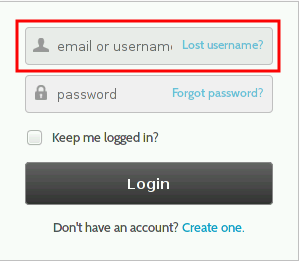
\includegraphics[width=0.8\textwidth]
      {../../images/eps/hubzero_login_page_username_field.png}
    \caption{Hub login form.}
    \label{fig:hubzero_login_page_username_html_2}
  \end{minipage}
\end{figure}

Take, for example, the hub login form shown in
\Cref{fig:hubzero_login_page_username_html_2}. The form contains a number of web
elements we would like to interact with, the most important of which are the
username field, password field, and login button.
\Cref{lst:hubzero_login_page_username_html} shows the HTML representation of the
username element in the login form.

Several of the locating strategies in Selenium can be used to identify the
element.  The examples in \Cref{tab:locatorMethods} show how this would be
done.  Among the available strategies, the ones involving the \xfparameter{id}
attribute are generally the most robust because HTML requires that the
id attribute be unique for all elements. This ensures that if the id attribute
exists for an element in the HTML DOM, then it should only exist once, reducing
the number of false positives when locating elements.

The locating strategies map directly to the Selenium WebDriver API functions
used to locate elements on the web page from a program. For the Python
bindings, these are a part of the \xfmethod{find\_element\_by\_*()} family of
methods shown in \Cref{lst:selenium_webdriver_find_element_functions}
Any one of these methods can be used to locate elements on a web page.

\begin{xcode}{%
  language=Python,%
  label=lst:selenium_webdriver_find_element_functions,%
  caption={The find\_elements\_by\_*() functions locate %
            web elements in Python.}%
}
# locating elements by the id attribute
element = browser.find_element_by_id('username')

# locating elements by name attribute
element = browser.find_element_by_name('username')

# locating elements by tag name
element = browser.find_element_by_tag_name('input')

# locating elements by XPath
element = browser.find_element_by_xpath("//input[@id='username']")

# locating elements by CSS Selector
element = browser.find_element_by_css_selector('input#username')
\end{xcode}

\subsection{Performing Actions on Web Elements}
\label{ssec:external_libs_selenium_performing_actions}

Once an element has been located, an action can be performed on the element.
Common actions include clicking on the element, sending key strokes to the
element, reading the properties of the element, and checking if the element is
displayed. \Cref{lst:selenium_webdriver_perform_actions_on_element}
demonstrates performing actions on the username field of the login web page.
In line 2, the username field is located using a CSS selector element locating
strategy. Lines 8 - 10 show that elements can be brought into focus on the web
page with the \xfmethod{click()} method, have its value erased using the
\xfmethod{clear()} method, and a new value assigned using the
\xfmethod{send\_keys()} method. By the end of this program, the username field on
the login page would be populated with the name ``hctest''.

\begin{xcode}{%
  language=Python,%
  label=lst:selenium_webdriver_perform_actions_on_element,%
  caption={Filling in the username field on the login form}%
}
# locate the username field by CSS Selector
element = browser.find_element_by_css('input#username')

# perform actions on the element:
# click the field to set focus
# clear any previous value from the field
# send key strokes to the field to fill in the username
element.click()
element.clear()
element.send_keys('hctest')
\end{xcode}

\subsection{Performing Mouse Actions on Web Elements}
\label{ssec:external_libs_selenium_mouse_actions}

In addition to being able to perform normal actions on elements, Selenium
WebDriver allows automation developers to perform mouse actions on elements
with a feature called ActionChains. ActionChains are useful for automating
tasks where a mouse movement is needed to trigger a property change in an
element on the web page. A common examples of this include JavaScript based
menus that appear on the screen when the mouse hovers over an element on the
web page, as shown in \Cref{fig:user_account_menu_closed}.

Selenium tries hard to only allow interaction with visible page elements that a
user would be able to interact with. If an element is present on the web page
and is available in the HTML DOM that the browser loaded, but is not visible to
the user, Selenium will not allow the automation code to perform actions on it.
Properties, like the text of the element or the attributes of its HTML, can
still be read, but clicking on the element or sending key strokes to the
element will fail.

To emulate the movement of the mouse, the automation developer can use Selenium
WebDriver's ActionChains.  ActionChains allow the automation developer to
specify elements on the web page to perform mouse actions on. ActionChains
support hovering the mouse over elements, single clicking elements, double
clicking elements, context (right) clicking elements, clicking and dragging
elements, and pressing a number of meta (ctrl, alt, shift) key combinations in
coordination with a mouse action.

\begin{figure}[htb]
        \centering
        \begin{subfigure}[b]{0.48\linewidth}
                \centering
%                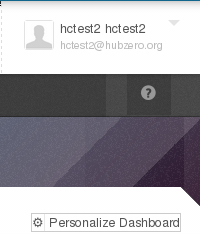
\includegraphics[width=0.5\textwidth]{../../images/corehubzero_javascripty_account_menu_closed.png}
                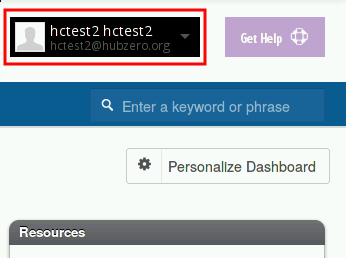
\includegraphics[width=\linewidth]{../../images/eps/nciphub_user_account_menu_closed.png}
                \caption{User account menu closed.}
                \label{fig:user_account_menu_closed}
        \end{subfigure}
        \begin{subfigure}[b]{0.48\linewidth}
                \centering
%                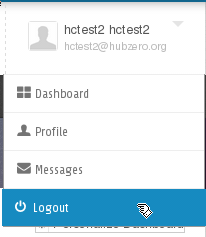
\includegraphics[width=0.5\textwidth]{../../images/corehubzero_javascripty_account_menu_open.png}
                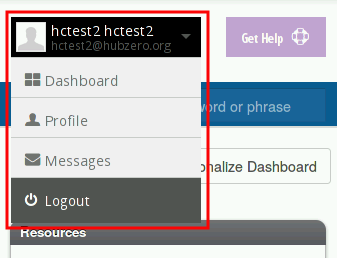
\includegraphics[width=\linewidth]{../../images/eps/nciphub_user_account_menu_open.png}
                \caption{User account menu open.}
                \label{fig:user_account_menu_open}
        \end{subfigure}
        \caption{Selenium WebDriver provides ActionChains to automate
                 performing mouse actions on elements of a web page.
                 ActionChains can be used for things like right or
                 left clicking on an element, drag and drop, and
                 hovering the mouse over an element.}
        \label{fig:action_chains_javascript_logout}
\end{figure}

On the hub, performing mouse actions is handy when trying to interact with the
user account menu, which requires the user to hover the mouse over the menu
element, shown in \Cref{fig:user_account_menu_closed}, in order to expose
account navigation options that lead to the user's Dashboard, Profile,
Messages, or log the user out of the website. To do this programmatically using
the Python bindings, an automation script would use the
\xfmodule{action\_chains} module.

\begin{xcode}{%
  language=Python,%
  label=lst:action_chains_javascript_logout_code,%
  caption={Activating a JavaScript menu using ActionChains.}%
}
# load the ActionChains class
from selenium.webdriver.common.action_chains import ActionChains

# locate the menu and logout elements by CSS Selector
menu_element = browser.find_element_by_css('#account')
logout_element = browser.find_element_by_css('#account-logout')

# build the ActionChains object to perform a mouse action:
# move the mouse over the menu to activate the JavaScript menu
# move the mouse to the logout list item in the menu
# single click the logout menu item
actionProvider = ActionChains(browser)
actionProvider.move_to_element(menu_element)
actionProvider.move_to_element(logout_element)
actionProvider.click()
actionProvider.perform()
\end{xcode}

Developers use the \xfclass{ActionChains} class to build (chain) a list of
actions together and send them to the web browser to be performed as if they
came from the computer's mouse.
\Cref{lst:action_chains_javascript_logout_code} demonstrates this by providing
a solution to the problem of hovering the mouse over the menu in
\Cref{fig:user_account_menu_closed}, exposing the account navigation options
shown in \Cref{fig:user_account_menu_open}. More specifically, the script
focuses on clicking the \xfhtmllink{Logout} link in the menu.

As with most Selenium WebDriver related scripting tasks, the first step is to
locate the web elements items the script will be interacting with in the HTML
DOM. Lines 5 and 6 of \Cref{lst:action_chains_javascript_logout_code}
are responsible for locating the menu element and the logout link on the web
page. Next, in lines 12 through 15, the script builds up a list of commands that
should be performed by the mouse. Each line in the script adds another command
that should be performed to the list stored in the variable
\xfparameter{actionProvider}. To get to the logout link, the mouse must first move
to the menu element, line 13, then move to the logout element, line 14, and
lastly send a click signal to press the logout link, line 15. The commands are
stored until the developer asks for them to be performed, shown in line 16 of
the script.


\subsection{Waiting for Web Elements}
\label{ssec:external_libs_selenium_waiting_for_elements}

% cite http://www.seleniumhq.org/docs/04_webdriver_advanced.jsp

Asynchronous JavaScript and XML (AJAX) is a programming technique that allows
web applications, running in the user's browser, to communicate with the web
server and dynamically change the state of the web application without
reloading the web page. The use of AJAX on web pages poses a problem for some
web automation software that evaluates static HTML DOMs without evaluating the
JavaScript that accompanies it.  After the browser makes a request for a web
page, the web server sends back a stream of HTML that can have JavaScript
embedded within it. The web browser is responsible for reading the HTML and
evaluating the JavaScript inside, which may request additional HTML from the
web server.

Selenium WebDriver uses the HTML and JavaScript engines inside of the external
web browser it is controlling to build the HTML DOM that represents the web
page the web browser loaded. This allows Selenium WebDriver to leverage the
same web browser to interpret and evaluate the HTML and JavaScript that a user
would.  This also adds a dimension of difficulty in locating web elements whose
presence or visibility on the web page is influenced by JavaScript. The dynamic
nature of JavaScript provides less structure to what it means for a web page to
have finished being `loaded'. Loading up multiple pieces of a web page may be
delayed, for example, by a slow network.  Selenium WebDriver provides two types
of waiting strategies, \textit{Implicit Waits} and \textit{Explicit Waits}, to
work around these unexpected delays and deal with locating elements that may
not be immediately available.

\subsubsection{Implicit Waits}
\label{sssec:external_libs_selenium_implicit_waits}

In Selenium WebDriver, the default behavior is to search once for a locator in
the HTML DOM.  If the locator cannot be found, a
\xfclass{NoSuchElementException} is raised. Implicit Waits are a way to
repeatedly search for a web element in the HTML DOM, while blocking other
commands from continuing, for a set amount of time before raising the
\xfclass{NoSuchElementException}.

Implicit waits can be setup once and exist for the life of the webdriver
object.  Setting up an implicit wait affects the whole family of
\xfmethod{find\_element*()} based methods, which will repeatedly search for the
element until either the element is found or the timeout limit is hit.

\subsubsection{Explicit Waits}
\label{sssec:external_libs_selenium_explicit_waits}

Explicit Waits consider the more general case where the automation developer
wants to wait for a condition to be met. Without explicit waits, many people
are tempted to check for the condition to be met while inside a \xfmethod{for}
loop, adding a call to the programming language's \xfmethod{sleep()} function
to space out the checks.  This approach should be avoided in favor of using the
\xfclass{WebdriverWait} class provided by the Selenium libraries.

% FIXME: add explicit wait example: submiting support ticket through the
%        need help interface.

\subsection{The Page Object Design Pattern}
\label{ssec:external_libs_selenium_page_objects}

The Page Object design pattern provides a layer of abstraction between a web
page and automation scripts. It represents the services offered on a web page
or a portion of a web page. By writing automation scripts that interact with
the page object, developers can significantly reduce the number of repeated
lines of code in their automation scripts, abstracting away many of the common
features of the code into a single class that needs to be updated as the web
page interface changes.

%Later on, we'll show how the use of the Page Objects design pattern helps
%reduce the size of the automation script, making it more readable, easier to
%write, and easier to maintain.


Novice developers learning to use Selenium for their web automation may start
by using the Selenium IDE, a graphical user interface product of the Selenium
project that records the actions of the user and stores them using an internal
representation called \textit{Selenese}. Selenium IDE also has the ability to
convert Selenese to a number of programming languages. The IDE allows
developers to quickly create automation scripts, but it suffers from the same
afflictions as manually writing automation scripts using the procedural
programming paradigm.  They both result in brittle scripts that break easily
and are painful to fix because of a lack of encapsulation.  With a little
organization and refactoring, these brittle scripts can be turned into robust
scripts that require less code to write and are easier to understand.

Consider the automation script in \Cref{lst:selenium_ide_hubzero_login},
which navigates the web browser to the \xfhtmllink{hubzero.org} web page,
clicks the link to login, then fills in the username field, fills in the
password field, and clicks the submit button.

\begin{xcode}{%
  language=Python,%
  label=lst:selenium_ide_hubzero_login,%
  caption={Simple hub login automation script.}%
}
from selenium import webdriver

# setup automation script constants
base_url = "http://hubzero.org/"

# start the browser
driver = webdriver.Firefox()

# navigate to the login page
driver.get(base_url)
driver.find_element_by_id("account-login").click()

# perform the login action
driver.find_element_by_css_selector("#username").clear()
driver.find_element_by_css_selector("#username").send_keys("abc")
driver.find_element_by_css_selector("#passwd").clear()
driver.find_element_by_css_selector("#passwd").send_keys("123")
driver.find_element_by_css_selector("[name='Submit']").click()
\end{xcode}


\noindent

Immediately looking at the code, a couple of patterns are apparent.  The first
pattern involves repeated searches for commonly used fields. This is true of
the field with id \xflocator{username}, which is searched for in line 14 to clear
it and again in line 15 to send it a value, and also for the the password field
with id \xflocator{passwd} for the same reasons in lines 16 and 17.  To clean up
this code, it could be rewritten to save the result of the first search to
a variable and call the \xfmethod{clear()} and \xfmethod{send\_keys()} methods on
that variable.

The second pattern involves the repeated steps used to populate a text field.
Every time a text field is populated, the script first searches for the
element, then clears the element of any previous value, and lastly, sends some
keys to the element. These actions could be combined into a function, as shown
in \Cref{lst:hubzero_login_utils} to help reduce the amount of repeated
code.

\begin{xcode}{%
  language=Python,%
  label=lst:hubzero_login_utils,%
  caption={populate\_input function included in utils.py}%
}
def populate_input(driver,loc,text):
  """type text into the element located by loc"""

  e = driver.find_element_by_css_selector(loc)
  e.clear()
  e.send_keys(text)
\end{xcode}

\noindent

An updated version of the automation script from
\Cref{lst:selenium_ide_hubzero_login} that addresses the first two patterns,
including a function named \xfmethod{populate\_input()} which finds an element
and types text into it, would look like this:

\begin{xcode}{%
  language=Python,%
  label=lst:hubzero_login_with_populate_input,%
  caption={Hub login script with repeated patterns abstracted away}%
}
from selenium import webdriver
from utils import populate_input

# setup automation script constants
base_url = "http://hubzero.org/"

# start the browser
driver = webdriver.Firefox()

# navigate to the login page
driver.get(base_url)
driver.find_element_by_css_selector("#account-login").click()

# perform the login action
populate_input(driver,"#username","abc")
populate_input(driver,"#passwd","123")
driver.find_element_by_css_selector("[name='Submit']").click()
\end{xcode}

At this point the automation script in
\Cref{lst:hubzero_login_with_populate_input} is looking pretty good. We were
able to abstract out most of the repeated code into a function,
\xfmethod{populate\_input()}, that we can pass arguments to and let it take
care of locating and writing text to elements of the HTML DOM. The act of
logging into the website has been condensed down to lines 15-17 in the
automation script, but this version of the automation script could still be
considered brittle.

Many web automation script errors are caused by failures to locate
elements in the HTML DOM.  This could be the result of poor element locator
strategy or just a new site design being implemented.  If multiple automation
scripts exist and they all repeat lines 15-17 from
\Cref{lst:hubzero_login_with_populate_input}, then they all need to be changed
to reflect the new design. The more scripts there are, the more painful the
processes of updating all of them is.

An alternative approach involves identifying common pieces of web pages that
can be interacted with and representing them as objects in code. The methods of
these objects are services provided by the web page. When the automation script
navigates to a web page, it would instantiate a page object, an object that
represents the web page, and call the page object's methods to perform actions
on that web page.

Applying the Page Object design pattern to the automation script in
\Cref{lst:hubzero_login_with_populate_input}, we first identify the web pages
being visited.  The first web page being visited is the hub's index page. On
the index page, the automation script locates and clicks the login link. The
first page object we create should represent the index page, and it should
provide the service of clicking the login link as one of its methods.
\Cref{lst:page_objects_generic_logged_out_page_v1} shows a page object representing a
generic web page where the user is logged out.

\begin{xcode}{%
  language=Python,%
  label=lst:page_objects_generic_logged_out_page_v1,%
  caption={A generic page object, providing the login navigation service.}%
}
class GenericLoggedOutPage(object):

  def __init__(self,driver):
    self.driver = driver

  def goto_login(self):
    """navigate to the login page"""

    self.driver.find_element_by_css_selector('#account-login').click()
\end{xcode}

\noindent

In \Cref{lst:page_objects_generic_logged_out_page_v1},
\xfclass{GenericLoggedOutPage} objects are initialized with a handle to the web
browser through the \xfparameter{driver} variable. The class has a method named
\xfmethod{goto\_login()} which provides an interface to the service of navigating
to the login web page by locating and clicking the login link.

After clicking the login link, the automation script in
\Cref{lst:hubzero_login_with_populate_input} fills in the login page web form
with a username and password, then clicks the submit button to complete the login
action. These commands can be grouped into another page object that represents
the login web page. In \Cref{lst:page_objects_login_page_v1}, the
\xfclass{LoginPage} page object provides the \xfmethod{login\_as()} method to
represent the service of filling in and submitting the login form.

\begin{xcode}{%
  language=Python,%
  label=lst:page_objects_login_page_v1,%
  caption={The Login page object represents the services provided by the login web page}%
}
from utils import populate_input

class LoginPage(object):

  def __init__(self,driver,loctype):
    self.driver = driver

  def login_as(self,username,password):
    """login a user by typing the username and password
       into the login form, and pressing the submit button
    """

    populate_input(driver,'#username',username)
    populate_input(driver,'#passwd',password)
    self.driver.find_element_by_css_selector("[name='Submit']").click()
\end{xcode}


\Cref{lst:hubzero_login_with_page_objects_v1} shows an updated version
of the automation script which incorporates the new page objects.  The updated
automation script puts more focus on the current web page and delegates the
steps to perform the actions to the page objects. The page objects can be used
in multiple automation scripts which promotes fewer lines of repeated code, and
cleaner looking, more readable automation scripts.  Additionally, all of the
actions for a particular web page are centralized in the page object.  When the
layout or locators for a web page change, only the page object needs to be
updated, provided the services of the web page don't change. This type of
encapsulation is one of the biggest advantages of the Page Object design
pattern.


\begin{xcode}{%
  language=Python,%
  label=lst:hubzero_login_with_page_objects_v1,%
  caption={Revised automation script, using Page Objects to perform actions.}%
}
from selenium import webdriver
from po_login import LoginPage
from po_generic_logged_out import GenericLoggedOutPage

# setup automation script constants
base_url = "http://hubzero.org/"
username = "abc"
password = "123"

# start the browser
driver = webdriver.Firefox()
driver.get(base_url)

# navigate to the login page
po = GenericLoggedOutPage(driver)
po.goto_login()

# perform the login action
po = LoginPage(driver)
po.login_as(username,password)
\end{xcode}


\section{BrowserMob Proxy}
\label{sec:external_libs_bmp}

Web browser automation tools provide functions to perform the actions a user
would manually perform inside of a web browser.  Beyond just automating the web
browser, writing programs to mimic the user experience sometimes requires
additional information about the result of a web request that is not always
apparent based on the elements available on the web page. Some of this
information can be gathered by using a web proxy in front of the browser.

% FIXME: add examples of what a web proxy would do

The purpose of the web proxy is to monitor and manipulate interactions between
the browser and web server. Because of its position as a man-in-the-middle, the
web proxy can record information about the requests from the web browser and
responses by the web server. The standard format used to store this type of
information is the HTTP Archive (HAR) format \cite{HAR12Format:Online}, now in
version 1.2.

% cite HAR format - http://www.softwareishard.com/blog/har-12-spec/
% cite BrowserMob Proxy - http://bmp.lightbody.net/
% cite BrowserMobProxy Python bindings - http://oss.theautomatedtester.co.uk/browsermob-proxy-py/

The BrowserMob Proxy \cite{BrowserMOBProxy:Online} is a web proxy that captures
the interactions of the web browser and the web server and reports it back to
the user in the HAR format. A separate project supplies Python language
bindings for communicating with the proxy server and starting new clients. The
BrowserMob Proxy fits in well with web browsers being controlled by Selenium
WebDriver.

The BrowserMob Proxy uses a single server to field requests for starting and
configuring proxies.  The server is started once and is responsible for
managing the proxies.  Separate proxy instances, referred to as clients, are
started for each browser.  Web requests are made by the browser and funneled
through the proxy client to the web server.

% cite RESTful? - https://en.wikipedia.org/wiki/Representational_state_transfer

The BrowserMob Proxy server provides a RESTful \cite{REST:Online} API that
allows users to programmatically control the server and proxy clients via
simple HTTP requests.  Since all of the server commands are HTTP requests, they
can be made using a program like \textbf{curl} \cite{Curl:Online}, a command
line utility for transferring data with URL syntax. The Python language
bindings \cite{BrowserMOBProxyPyBindings:Online}, which were developed by a
third party, provide similar functionality.  \Cref{lst:bmp_startup_and_request}
demonstrates how to start the proxy and attach it to a Selenium WebDriver
controlled web browser.

\begin{xcode}{%
  language=Python,%
  label=lst:bmp_startup_and_request,%
  caption={Starting the BrowserMob Proxy server and client}%
}
from selenium import webdriver
import browsermobproxy

bmp_path = '/usr/local/bin/browsermob-proxy'

proxy_server = browsermobproxy.Server(bmp_path,{'port':9090})
proxy_server.start()

# start up a proxy client
proxy_client = proxy_server.create_proxy()

# block any requests to facebook
proxy_client.blacklist('http(s)?://.*facebook\\.com/?.*',200)

# launch a browser, setting the proxy, load a web page
browser = webdriver.Firefox(proxy=proxy_client)
browser.get('https://hubzero.org')

# get the har of the last request from the browser
har = proxy_client.har

# close down the proxy server and client
proxy_client.close()
proxy_server.stop()
\end{xcode}


%client, associate it with a Selenium WebDriver controlled web browser, and load
%the resulting HAR file after requesting a web page.

% cite https://github.com/AutomatedTester/browsermob-proxy-py

%\subsection{Starting the server}
%\subsection{Starting a proxy client}
%\subsection{Configuring the proxy client}
%\subsection{Connecting the web browser to the proxy}

\section{Paramiko}
\label{sec:external_libs_paramiko}

% cite http://www.lag.net/paramiko/ cite https://github.com/paramiko/paramiko

Paramiko \cite{Paramiko:Online} is a Python based implementation of the SSH
version 2 protocol for making secure connections between machines.  Using
Paramiko, users can programmatically open secure channels for access to
services on remote machines including shells and SFTP.

\begin{xcode}{%
  language=Python,%
  label=fig:paramiko_intro,%
  caption={Starting a SSH and SFTP connection using the Paramiko library.}%
}
import paramiko

# setup the SSH client and authenticate
client = paramiko.SSHClient()
client.set_missing_host_key_policy(paramiko.AutoAddPolicy())
client.load_system_host_keys()
client.connect(
    hostname='hubzero.org',
    port=22,
    username='user1',
    password='user1password')

# execute a single command
stdin, stdout, stderr = client.exec_command('ls')

# invoke a new shell and execute multiple commands
channel = client.invoke_shell(width=1000,height=1000)

# start up an SFTP channel
transport = client.get_transport()
sftp = paramiko.SFTPClient.from_transport(transport)
\end{xcode}


%\subsection{Opening a secure shell connection}
%\subsection{Communicating over a connection}


